\begin{frame}{Расчёт характеристик монёвренности}{Задачи раздела}
    \begin{block}{Задачи}
        Расчёт:
        \begin{itemize}
            \item Нормальной перегрузки на вираже $n_{y_\text{вир}}$
            \item Угловой скорости на вираже $\omega_\text{вир}$
            \item Времени выполнение виража $t_\text{вир}$
            \item Радиуса на вираже $r_\text{вир}$
        \end{itemize}
    \end{block}
\end{frame}

\begin{frame}{Расчёт характеристик манёвренности}{Графики}
    \begin{minipage}[c]{0.45\textwidth}
        \center{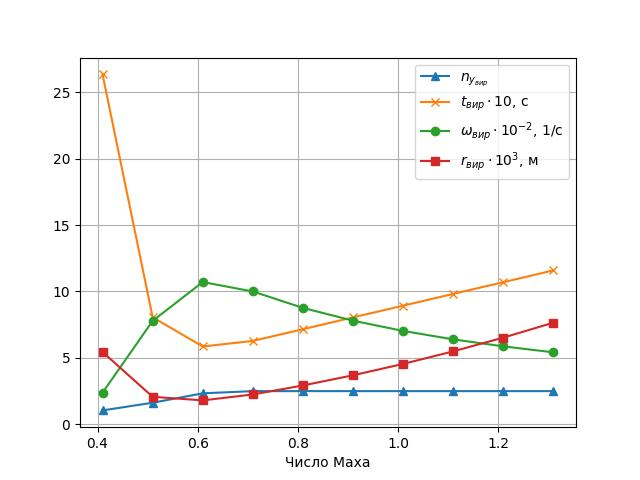
\includegraphics[width=6cm, height = 7cm]{../Оглавление/Part1/figures/РезультатыМаневры.jpg}}
    \end{minipage}  
    \begin{minipage}[c]{0.45\textwidth}
        \center{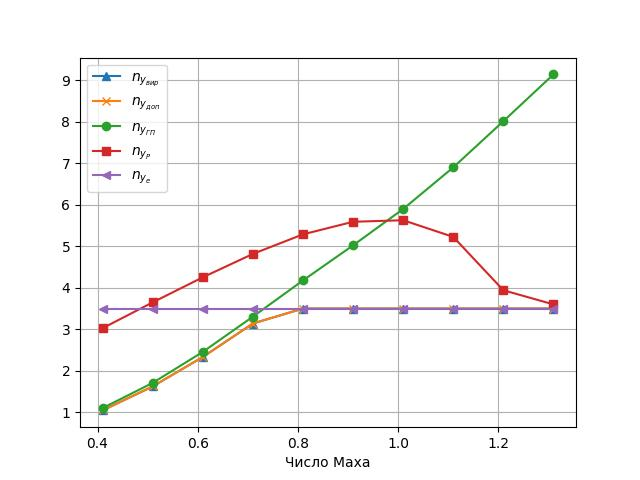
\includegraphics[width=6cm, height = 7cm]{../Оглавление/Part1/figures/РезультатыМаневры2.jpg}}
    \end{minipage}
\end{frame}